\PassOptionsToPackage{table}{xcolor}
\documentclass[12pt,letterpaper,twocolumn,openany,nodeprecatedcode,bg=none]{dndbook}
\usepackage[english]{babel}
\usepackage[utf8]{inputenc}
\usepackage{longtable,booktabs,array}
\usepackage{calc}
\usepackage{etoolbox}
\usepackage{caption}
\usepackage{float}
\usepackage{graphicx}
\usepackage{needspace}
\usepackage{tikz}

% Reset zebra striping at the start of every table
\AtBeginEnvironment{longtable}{\rowcolors{1}{white}{gray!10}\small}
\AtBeginEnvironment{table}{\rowcolors{1}{white}{gray!10}}

\providecommand{\pandocbounded}[1]{#1}
\providecommand{\tightlist}{%
  \setlength{\itemsep}{0pt}\setlength{\parskip}{0pt}}

\captionsetup{labelformat=empty}
\setcounter{secnumdepth}{0}
\setlength{\parindent}{0pt}
\setlength{\parskip}{0.5\baselineskip}
\setlength{\headheight}{15pt}

% Prevent orphaned subsections
\let\oldsubsection\subsection
\renewcommand{\subsection}[1]{%
  \needspace{5\baselineskip}%
  \oldsubsection{#1}%
}

\begin{document}
\onecolumn

      \title{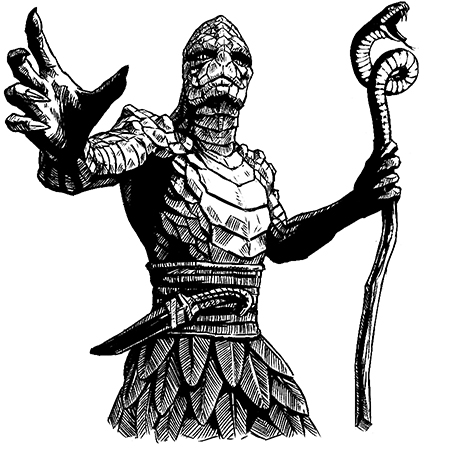
\includegraphics[width=0.9\textwidth,height=0.55\textheight,keepaspectratio]{lizardDruid.jpg}\\[1.5cm]Druid}
  \author{Class Handbook}
\date{}
\maketitle



\clearpage
\twocolumn

\section{Druid}\label{druid}

\subsection{Core Druid Traits}\label{core-druid-traits}

\needspace{11\baselineskip}

{\def\LTcaptype{none} % do not increment counter
\begin{table}[!htbp]
\centering
\begin{tabular}{@{}
  >{\raggedright\arraybackslash}p{(\linewidth - 2\tabcolsep) * \real{0.3824}}
  >{\raggedright\arraybackslash}p{(\linewidth - 2\tabcolsep) * \real{0.6176}}@{}}
\toprule\noalign{}
\begin{minipage}[b]{\linewidth}\raggedright
\textbf{Primary Ability}
\end{minipage} & \begin{minipage}[b]{\linewidth}\raggedright
Wisdom
\end{minipage} \\
\midrule\noalign{}
\textbf{Hit Points} & 1d4 \\
\textbf{Saving Throw Proficiencies} & Intelligence, Wisdom \\
\textbf{Skill Proficiencies} & Choose 2 skills \\
\textbf{Weapon Proficiencies} & Choose 1 category \\
\textbf{Starting Equipment} & Padded Jacket, Robe, Staff, Thorny
Circlet \\
\bottomrule\noalign{}
\end{tabular}
\end{table}
}

\subsection{Druid Features}\label{druid-features}

\needspace{20\baselineskip}

{\def\LTcaptype{none} % do not increment counter
\begin{table}[!htbp]
\centering
\begin{tabular}{@{}
  >{\raggedright\arraybackslash}p{(\linewidth - 4\tabcolsep) * \real{0.0962}}
  >{\raggedright\arraybackslash}p{(\linewidth - 4\tabcolsep) * \real{0.2115}}
  >{\raggedright\arraybackslash}p{(\linewidth - 4\tabcolsep) * \real{0.6923}}@{}}
\toprule\noalign{}
\begin{minipage}[b]{\linewidth}\raggedright
Level
\end{minipage} & \begin{minipage}[b]{\linewidth}\raggedright
Proficiency
\end{minipage} & \begin{minipage}[b]{\linewidth}\raggedright
Class Features
\end{minipage} \\
\midrule\noalign{}
1 & +2 & Spellcasting, Wild Shape, Beast Bond \\
2 & +2 & --- \\
3 & +2 & Ability Bonus \\
4 & +2 & --- \\
5 & +2 & --- \\
6 & +2 & --- \\
7 & +2 & Ability Bonus \\
8 & +2 & --- \\
9 & +3 & --- \\
10 & +3 & --- \\
\bottomrule\noalign{}
\end{tabular}
\end{table}
}

\subsection{Level 1: Spellcasting}\label{level-1-spellcasting}

You can cast spells from the Druid spell list. Wisdom is your casting
ability. You know two cantrips.

You prepare a number of spells equal to your Intelligence modifier. You
may change your prepared spells after an extended period of downtime.

You regain all expended spell slots when you finish a long rest. Once
per day, you may regain 1 expended spell slot when you finish a short
rest.

\subsection{Spell Slots by Level}\label{spell-slots-by-level}

\needspace{20\baselineskip}

{\def\LTcaptype{none} % do not increment counter
\begin{table}[!htbp]
\centering
\begin{tabular}{@{}
  >{\raggedright\arraybackslash}p{(\linewidth - 6\tabcolsep) * \real{0.3571}}
  >{\raggedright\arraybackslash}p{(\linewidth - 6\tabcolsep) * \real{0.2143}}
  >{\raggedright\arraybackslash}p{(\linewidth - 6\tabcolsep) * \real{0.2143}}
  >{\raggedright\arraybackslash}p{(\linewidth - 6\tabcolsep) * \real{0.2143}}@{}}
\toprule\noalign{}
\begin{minipage}[b]{\linewidth}\raggedright
Level
\end{minipage} & \begin{minipage}[b]{\linewidth}\raggedright
1
\end{minipage} & \begin{minipage}[b]{\linewidth}\raggedright
2
\end{minipage} & \begin{minipage}[b]{\linewidth}\raggedright
3
\end{minipage} \\
\midrule\noalign{}
1 & 2 & -- & -- \\
2 & 2 & -- & -- \\
3 & 3 & -- & -- \\
4 & 3 & -- & -- \\
5 & 4 & 2 & -- \\
6 & 4 & 2 & -- \\
7 & 4 & 3 & -- \\
8 & 4 & 3 & -- \\
9 & 4 & 3 & 2 \\
10 & 4 & 3 & 2 \\
\bottomrule\noalign{}
\end{tabular}
\end{table}
}

\subsection{Level 1: Wild Shape}\label{level-1-wild-shape}

As an action, you can transform into a beast you have seen. While
transformed, you use the beast's AC, hit points, and Speed, but retain
your Intelligence, Wisdom, and Charisma, and your spellcasting ability.
If you are reduced to 0 HP while in your beast form, you return to your
human form with your prior HP, taking any excess damage. You also take a
death saving throw failure. You can't cast spells while transformed.

You can remain transformed for up to 1 hour, and you can transform back
as an action. Once you use this feature, you can't use it again until
you finish a short rest.

Several beast forms are detailed at the bottom of the class description.
A form requires the druid be a certain level to transform into them.
When you transform, any non-metal items you are wearing or carrying can
meld into your new form, while metallic items drop to the ground.

\subsection{Level 1: Beast Bond}\label{level-1-beast-bond}

Your druidic magic has taught you how to perform a ritual that will
grant you the ability to speak with animals. You must perform a ritual
that takes 1 minute in order to activate this ability, which then lasts
for 1 hour.

\subsection{Level 3: Ability Bonus}\label{level-3-ability-bonus}

You gain a +1 bonus to two different abilities of your choice.

\subsection{Level 7: Ability Bonus}\label{level-7-ability-bonus}

You gain a +1 bonus to two different abilities of your choice.

\section{Wild Shape Forms}\label{wild-shape-forms}

Each form lists a level. You can only transform into a form whose level
is less than or equal to your druid level.

\textbf{Damage.} The feature lists the damage dice an attack uses. You
also may add the form's Strength or Dexterity modifier to the roll,
whichever is higher.

\textbf{Saving Throws.} The saving throw DC of any beast form feature
that requires one is 8 + your Wisdom modifier + your proficiency bonus.

\newpage

\subsection{Wolf}\label{wolf}

\begin{quote}
\textbf{\emph{Level 1 Form}}
\end{quote}

\needspace{15\baselineskip}

{\def\LTcaptype{none} % do not increment counter
\begin{table}[!htbp]
\centering
\begin{tabular}{@{}
  >{\centering\arraybackslash}p{(\linewidth - 2\tabcolsep) * \real{0.6667}}
  >{\centering\arraybackslash}p{(\linewidth - 2\tabcolsep) * \real{0.3333}}@{}}
\toprule\noalign{}
\begin{minipage}[b]{\linewidth}\centering
Stat
\end{minipage} & \begin{minipage}[b]{\linewidth}\centering
Value
\end{minipage} \\
\midrule\noalign{}
HP & 11 \\
AC & 12 \\
Speed & 40 ft. \\
Size & Medium \\
Strength & +2 \\
Dexterity & +2 \\
Constitution & +1 \\
\bottomrule\noalign{}
\end{tabular}
\end{table}
}

\textbf{Prowling Hunter.} You have advantage on Perception and Stealth
checks.

\textbf{Perfect Senses.} As an action on your turn, you can hone your
senses. For the next minute, you can see invisible objects and creatures
and detect hidden creatures that are within 30 feet of you. This benefit
applies only while in this form.

\textbf{Bite.} Your bite does 1d8 piercing damage.

\subsection{Rat}\label{rat}

\begin{quote}
\textbf{\emph{Level 1 Form}}
\end{quote}

\needspace{15\baselineskip}

{\def\LTcaptype{none} % do not increment counter
\begin{table}[!htbp]
\centering
\begin{tabular}{@{}
  >{\centering\arraybackslash}p{(\linewidth - 2\tabcolsep) * \real{0.3750}}
  >{\centering\arraybackslash}p{(\linewidth - 2\tabcolsep) * \real{0.6250}}@{}}
\toprule\noalign{}
\begin{minipage}[b]{\linewidth}\centering
Stat
\end{minipage} & \begin{minipage}[b]{\linewidth}\centering
Value
\end{minipage} \\
\midrule\noalign{}
HP & 6 \\
AC & 13 \\
Speed & 20 ft., climb 20 ft. \\
Size & Tiny \\
Strength & -3 \\
Dexterity & +3 \\
Constitution & 0 \\
\bottomrule\noalign{}
\end{tabular}
\end{table}
}

\textbf{Sewer Sneak.} You have advantage on Stealth checks and have
expertise with them.

\textbf{Bite.} Your bite does 1d4 piercing damage.

\subsection{Fish}\label{fish}

\begin{quote}
\textbf{\emph{Level 2 Form}}
\end{quote}

\needspace{15\baselineskip}

{\def\LTcaptype{none} % do not increment counter
\begin{table}[!htbp]
\centering
\begin{tabular}{@{}
  >{\centering\arraybackslash}p{(\linewidth - 2\tabcolsep) * \real{0.4000}}
  >{\centering\arraybackslash}p{(\linewidth - 2\tabcolsep) * \real{0.6000}}@{}}
\toprule\noalign{}
\begin{minipage}[b]{\linewidth}\centering
Stat
\end{minipage} & \begin{minipage}[b]{\linewidth}\centering
Value
\end{minipage} \\
\midrule\noalign{}
HP & 4 \\
AC & 15 \\
Speed & 5 ft., swim 40 ft. \\
Size & Tiny \\
Strength & -3 \\
Dexterity & +4 \\
Constitution & 0 \\
\bottomrule\noalign{}
\end{tabular}
\end{table}
}

\textbf{Aquatic.} You can breathe water.

\textbf{Bite.} Your bite does 1 piercing damage.

\subsection{Bird}\label{bird}

\begin{quote}
\textbf{\emph{Level 4 Form}}
\end{quote}

\needspace{15\baselineskip}

{\def\LTcaptype{none} % do not increment counter
\begin{table}[!htbp]
\centering
\begin{tabular}{@{}
  >{\centering\arraybackslash}p{(\linewidth - 2\tabcolsep) * \real{0.4000}}
  >{\centering\arraybackslash}p{(\linewidth - 2\tabcolsep) * \real{0.6000}}@{}}
\toprule\noalign{}
\begin{minipage}[b]{\linewidth}\centering
Stat
\end{minipage} & \begin{minipage}[b]{\linewidth}\centering
Value
\end{minipage} \\
\midrule\noalign{}
HP & 3 \\
AC & 15 \\
Speed & 10 ft., fly 60 ft. \\
Size & Tiny \\
Strength & -3 \\
Dexterity & +4 \\
Constitution & 0 \\
\bottomrule\noalign{}
\end{tabular}
\end{table}
}

\textbf{Talons.} Your talons do 1d4 slashing damage.

\newpage

\subsection{Bear}\label{bear}

\begin{quote}
\textbf{\emph{Level 8 Form}}
\end{quote}

\needspace{15\baselineskip}

{\def\LTcaptype{none} % do not increment counter
\begin{table}[!htbp]
\centering
\begin{tabular}{@{}
  >{\centering\arraybackslash}p{(\linewidth - 2\tabcolsep) * \real{0.6667}}
  >{\centering\arraybackslash}p{(\linewidth - 2\tabcolsep) * \real{0.3333}}@{}}
\toprule\noalign{}
\begin{minipage}[b]{\linewidth}\centering
Stat
\end{minipage} & \begin{minipage}[b]{\linewidth}\centering
Value
\end{minipage} \\
\midrule\noalign{}
HP & 32 \\
AC & 13 \\
Speed & 40 ft. \\
Size & Large \\
Strength & +4 \\
Dexterity & +1 \\
Constitution & +2 \\
\bottomrule\noalign{}
\end{tabular}
\end{table}
}

\textbf{Roaring Guardian.} Once per short rest, you can use an action to
regain 2d6 + your spellcasting modifier hit points and goad hostile
creatures within 15 feet of you for 1 round.

\textbf{Bite.} Your bite does 2d6 piercing damage.

\textbf{Claws.} Your claws do 1d8 slashing damage.

\textbf{Multiattack.} As an attack action, you can attack with your bite
and your claws. At level 9, you can bite once and attack with your claws
twice.

\newpage

\subsection{Sabre Tooth Tiger}\label{sabre-tooth-tiger}

\begin{quote}
\textbf{\emph{Level 10 Form}}
\end{quote}

\needspace{15\baselineskip}

{\def\LTcaptype{none} % do not increment counter
\begin{table}[!htbp]
\centering
\begin{tabular}{@{}
  >{\centering\arraybackslash}p{(\linewidth - 2\tabcolsep) * \real{0.6667}}
  >{\centering\arraybackslash}p{(\linewidth - 2\tabcolsep) * \real{0.3333}}@{}}
\toprule\noalign{}
\begin{minipage}[b]{\linewidth}\centering
Stat
\end{minipage} & \begin{minipage}[b]{\linewidth}\centering
Value
\end{minipage} \\
\midrule\noalign{}
HP & 42 \\
AC & 13 \\
Speed & 50 ft. \\
Size & Large \\
Strength & +4 \\
Dexterity & +3 \\
Constitution & +2 \\
\bottomrule\noalign{}
\end{tabular}
\end{table}
}

\textbf{Relentless Hunter.} Once per short rest, you can move up to
twice your speed without provoking opportunity attacks, and attacks
against you have disadvantage until the start of your next turn.

\textbf{Bite.} Your bite does 4d6 piercing damage.

\textbf{Claws.} Your claws do 1d10 slashing damage.

\textbf{Multiattack.} As an attack action, you can attack with your bite
and your claws.

\section{Druid Spells}\label{druid-spells}

The tables are numbered to allow quick generation of spells known for a
new character.

\subsection{Cantrips}\label{cantrips}

\needspace{9\baselineskip}

{\def\LTcaptype{none} % do not increment counter
\begin{table}[!htbp]
\centering
\begin{tabular}{@{}
  >{\raggedright\arraybackslash}p{(\linewidth - 2\tabcolsep) * \real{0.2000}}
  >{\raggedright\arraybackslash}p{(\linewidth - 2\tabcolsep) * \real{0.8000}}@{}}
\toprule\noalign{}
\begin{minipage}[b]{\linewidth}\raggedright
d4
\end{minipage} & \begin{minipage}[b]{\linewidth}\raggedright
Cantrip
\end{minipage} \\
\midrule\noalign{}
1 & Light \\
2 & Mending \\
3 & Ray of Frost \\
4 & Thaumaturgy \\
\bottomrule\noalign{}
\end{tabular}
\end{table}
}

\subsection{Level 1 Spells}\label{level-1-spells}

\needspace{9\baselineskip}

{\def\LTcaptype{none} % do not increment counter
\begin{table}[!htbp]
\centering
\begin{tabular}{@{}
  >{\raggedright\arraybackslash}p{(\linewidth - 2\tabcolsep) * \real{0.2000}}
  >{\raggedright\arraybackslash}p{(\linewidth - 2\tabcolsep) * \real{0.8000}}@{}}
\toprule\noalign{}
\begin{minipage}[b]{\linewidth}\raggedright
d4
\end{minipage} & \begin{minipage}[b]{\linewidth}\raggedright
Level 1
\end{minipage} \\
\midrule\noalign{}
1 & Cure Wounds \\
2 & Detect Magic \\
3 & Entangle \\
4 & Wall of Fog \\
\bottomrule\noalign{}
\end{tabular}
\end{table}
}

\subsection{Level 2 Spells}\label{level-2-spells}

\needspace{9\baselineskip}

{\def\LTcaptype{none} % do not increment counter
\begin{table}[!htbp]
\centering
\begin{tabular}{@{}
  >{\raggedright\arraybackslash}p{(\linewidth - 2\tabcolsep) * \real{0.1500}}
  >{\raggedright\arraybackslash}p{(\linewidth - 2\tabcolsep) * \real{0.8500}}@{}}
\toprule\noalign{}
\begin{minipage}[b]{\linewidth}\raggedright
d4
\end{minipage} & \begin{minipage}[b]{\linewidth}\raggedright
Level 2
\end{minipage} \\
\midrule\noalign{}
1 & Levitate \\
2 & Restorative Touch \\
3 & See Invisibility \\
4 & Silence \\
\bottomrule\noalign{}
\end{tabular}
\end{table}
}

\subsection{Level 3 Spells}\label{level-3-spells}

\needspace{9\baselineskip}

{\def\LTcaptype{none} % do not increment counter
\begin{table}[!htbp]
\centering
\begin{tabular}{@{}
  >{\raggedright\arraybackslash}p{(\linewidth - 2\tabcolsep) * \real{0.1667}}
  >{\raggedright\arraybackslash}p{(\linewidth - 2\tabcolsep) * \real{0.8333}}@{}}
\toprule\noalign{}
\begin{minipage}[b]{\linewidth}\raggedright
d4
\end{minipage} & \begin{minipage}[b]{\linewidth}\raggedright
Level 3
\end{minipage} \\
\midrule\noalign{}
1 & Fly \\
2 & Lightning Bolt \\
3 & Revivify \\
4 & Water Breathing \\
\bottomrule\noalign{}
\end{tabular}
\end{table}
}

\newpage

\section{Druid Spell List}\label{druid-spell-list}

Spells descriptions are listed below.

\subsection{Cure Wounds}\label{cure-wounds}

\textbf{Level:} 1

\textbf{Range:} Touch

A creature you touch regains 2d8 + your spellcasting bonus hit points.

The healing increases to 4d8 + your spellcasting bonus if you use a
level 2 slot and 6d8 + your spellcasting bonus if you use a level 3
slot.

\subsection{Detect Magic}\label{detect-magic}

\textbf{Level:} 1

\textbf{Range:} Self

\textbf{Duration:} Concentration, up to 10 minutes

You see the presence of magical effects within 30 feet on objects that
are visible to you. Magic appears as a faint aura, the details of which
allow you to determine its origin and the basic details of its effect.

\subsection{Entangle}\label{entangle}

\textbf{Level:} 1

\textbf{Range:} 90 feet

\textbf{Duration:} Concentration, up to 1 minute

Grasping plants sprout from the ground in a 20-foot square within range.
For the duration, these plants turn the ground in the area into
difficult terrain. They disappear when the spell ends. Each creature
(other than you) in the area when you cast the spell must succeed on a
Strength saving throw or have the restrained condition until the spell
ends.

A restrained creature can take an action on their turn to repeat the
save. On a success, it frees itself from the grasping plants and is no
longer restrained by them.

\subsection{Fly}\label{fly}

\textbf{Level:} 3

\textbf{Range:} Touch

\textbf{Duration:} Concentration, up to 10 minutes

You touch a willing creature. For the duration, the target gains a fly
speed.

When the spell ends, the target falls if it is still aloft unless it can
stop the fall.

\subsection{Levitate}\label{levitate}

\textbf{Level:} 2

\textbf{Range:} 60 feet

\textbf{Duration:} Concentration, up to 10 minutes

One creature or loose object of your choice within range rises
vertically up to 20 feet and remains suspended there. The spell can
levitate an object that weighs up to 500 pounds. An unwilling creature
that succeeds on a Constitution saving throw is unaffected.

The target can move only by pushing or pulling against a fixed object or
surface within reach (such as a wall or a ceiling), which allows it to
move as if it were climbing. You can change the target's altitude by up
to 20 feet in either direction on your turn. If you are the target, you
can move up or down as part of your move. Otherwise, you can take an
action to move the target, which must remain within the spell's range.

When the spell ends, the target floats gently to the ground if it is
still aloft.

\subsection{Light}\label{light}

\textbf{Level:} Cantrip

\textbf{Range:} Touch

\textbf{Duration:} 1 hour

An object you touch sheds dim light in a 30-foot radius and Dim Light
for an additional 20 feet. The spell ends if you cast it again.

\subsection{Lightning Bolt}\label{lightning-bolt}

\textbf{Level:} 3

\textbf{Range:} 300 feet

You can make ranged spell attacks against up to three targets. The
damage is 6d10 lightning damage if you attack three targets, 8d10
lightning damage if you attack two, or 10d10 lightning damage if you
attack one. If the attack misses, the target takes half damage.

\subsection{Mending}\label{mending}

\textbf{Level:} Cantrip

\textbf{Range:} Touch

This spell repairs a single break or tear in an object you touch. If the
break or tear is no larger than 1 foot in any dimension, you mend it,
leaving no trace of the former damage.

\subsection{Ray of Frost}\label{ray-of-frost}

\textbf{Level:} Cantrip

\textbf{Range:} 60 feet

A frigid beam of blue-white light streaks toward a creature within
range. Make a ranged spell attack against the target. On a hit, it takes
1d8 cold damage, and its speed is reduced by 20 feet until after its
next turn.

The damage increases to 2d8 cold damage at level 5 and 3d8 cold damage
at level 9.

\subsection{Restorative Touch}\label{restorative-touch}

\textbf{Level:} 2

\textbf{Range:} Touch

You touch a creature and end one condition on it: blinded, paralyzed, or
poisoned.

\subsection{Revivify}\label{revivify}

\textbf{Level:} 3

\textbf{Range:} Touch

You touch a creature. If that creature died within the last minute, it
returns to life, restores one failed death save, and regains 1 hit
point. It cannot restore failed death saves again until it finishes a
long rest.

\subsection{See Invisibility}\label{see-invisibility}

\textbf{Level:} 2

\textbf{Range:} Self

\textbf{Duration:} 1 hour

You see creatures and objects that are invisible as if they were
visible.

\subsection{Silence}\label{silence}

\textbf{Level:} 2

\textbf{Range:} 120 feet

\textbf{Duration:} Concentration, up to 10 minutes

No sound can be created within or pass through a 20-foot-radius sphere
centered on a point you choose within range. Any creature or object
entirely inside the sphere has immunity to thunder damage. Spells cannot
be cast in the spell's area.

\subsection{Thaumaturgy}\label{thaumaturgy}

\textbf{Level:} Cantrip

\textbf{Range:} 30 feet

\textbf{Duration:} Up to 1 minute

You manifest a minor wonder within range. You can create minor
illusions, alter one of your physical traits, change the sound or volume
of your voice, and otherwise make cosmetic changes to yourself or an
object in range. The spell ends if you cast it again.

\subsection{Wall of Fog}\label{wall-of-fog}

\textbf{Level:} 1

\textbf{Range:} 120 feet

\textbf{Duration:} 10 minutes

You create a thick, billowing wall of fog that blocks sight and sound.
It is one-foot thick, 10 feet high, and up to 30 feet long. The wall can
bend and turn as you wish, but all of it must be within the spell's
range when you create it.

\subsection{Water Breathing}\label{water-breathing}

\textbf{Level:} 3

\textbf{Range:} 30 feet

\textbf{Duration:} 24 hours

This spell grants up to ten willing creatures of your choice within
range the ability to breathe underwater until the spell ends. Affected
creatures also retain their normal mode of respiration.

\onecolumn

\clearpage
\thispagestyle{empty}
\begin{center}
\vspace*{\fill}
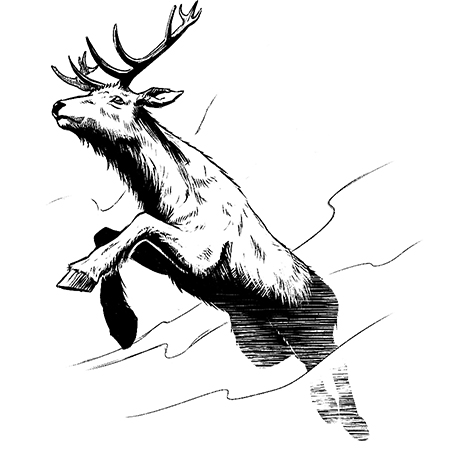
\includegraphics[width=0.7\textwidth,keepaspectratio]{elk.jpg}\par
\vspace{0.4cm}
{\itshape Nature shall rise against you.}\par
\vspace*{\fill}
\end{center}

\end{document}